\chapter{Hadoop}

Atualmente, o Google é uma empresa de consulta e publicidade e é capaz de fornecer os seus serviços devido a investimentos em armazenamento distribuído em larga escala e a capacidade de processamento, estes desenvolvidos \emph{in-house}.

Essa capacidade é fornecida por um grande número de PCs, pelo Google File System (GFS), um sistema de arquivos redundantes em \emph{cluster}, pelo sistema operacional GNU/Linux e pelo MapReduce, um \emph{middleware} de processamento paralelo de dados.

Em 2004, um artigo~\cite{Dean:2004}, que foi publicado por
profissionais da Google, propôs o MapReduce. Em 2006, estes
profissionais, juntamente com Doug Cutting do Yahoo!, formaram um
sub-projeto do Apache Lucene\footnote{http://www.apache.org} que foi
chamado Hadoop\footnote{http://hadoop.apache.org/}.

Mais recentemente, o projeto Apache Hadoop tem desenvolvido uma
reimplementação de partes do GFS e MapReduce e muitos grupos da
comunidade de software livre posteriormente abraçaram essa tecnologia,
permitindo-lhes fazer coisas que eles não poderiam fazer em máquinas
individuais. O Hadoop está disponível em código fonte sob
licenciamento Apache \emph{license} (compatível com GPL).

O Hadoop é um \emph{framework} para executar aplicações em
armazenamento distribuído de grande volume de dados que pode ser
construído com \emph{commodity hardware}, que é facilmente acessível e
disponível.  O Hadoop não é um \emph{framework} canônico. Ele foi
projetado para aplicações que atualizam dados da seguinte forma: uma
escrita e muitas leituras, através de acessos por \emph{batch}, com
tamanho da ordem de petabytes, organizados de forma não estruturada,
com esquema dinâmico e integridade baixa.  Uma lista de aplicações e
organizações que usam o Hadoop pode ser encontrada em
\cite{HadoopWiki:2010}.

Em poucas palavras, o Hadoop disponibiliza um armazenamento
compartilhado (HDFS) e um sistema de análise (MapReduce) que compõem o
seu \emph{kernel}.

\section{MapReduce}

O MapReduce utiliza algoritmos de ordenação para reconstruir sua base de dados.  Um bom uso para o MapReduce são aplicações cujos dados são escritos uma vez e lidos muitas vezes. São dados não estruturados como texto ou imagens. O MapReduce tenta colocar esses dados no nó onde são feitas as computações, desta forma, o acesso aos dados é rápido, pois é local \cite{White:2009}.

O MapReduce pode resolver problemas genéricos, cujos dados podem ser divididos em matrizes de dados, para cada matriz a mesma computação necessária (sub-problema) e não existe necessidade de comunicação entre as tarefas (sub-problemas). A execução de um típico \emph{job} do MapReduce pode ser assim descrita:

\begin{itemize}
    \item Iteração sobre um número grande de registros
    \item Map extrai algo de cada registro (chave, valor)
    \item Rearranjo (\emph{shuffle}) e ordenação de resultados intermediários por (chave, valor)
    \item Reduce agrega os resultados intermediários
    \item Geração da saída
\end{itemize}

Um programas para execução no HDFS/MapReduce que podem ser escritos em várias linguagens como Java, Ruby, Python e C++.


\section{Arquitetura do Hadoop \emph{Distributed File System}}

Um \emph{cluster} do HDFS é composto por um único NameNode, um
servidor-mestre que gerencia o sistema de arquivos e controla o acesso
aos arquivos de clientes. Há uma série de DataNodes, geralmente um por
nó do \emph{cluster}, que gerenciam o armazenamento anexado ao nó em
que são executados. A Figura~\ref{fig6:hfs} mostra o NameNode e os
DataNodes.

Uma típica arquitetura de rede em dois níveis para um \emph{cluster}
Hadoop é construída por vários \emph{racks} interligados por um
comutador como mostra a Figura~\ref{fig5:hc}. Cada \emph{rack} por sua
vez é formado por vários nós (máquinas) e seus discos, estes também
interligados por um comutador.

    \vspace*{2cm}
    \begin{figure}[h]
      \centering
      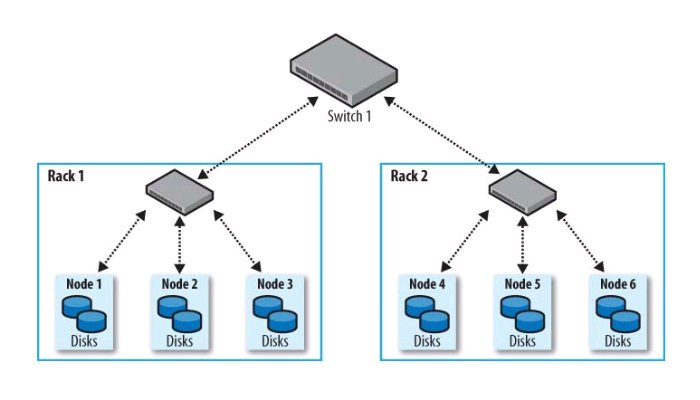
\includegraphics[scale=0.6]{figuras/hadoop-cluster.jpg}
      \caption{Arquitetura de rede em dois níveis para um cluster Hadoop~\cite{Hadoop:2010}}
      \label{fig5:hc}
    \end{figure} 

O NameNode executa operações no sistema de arquivos, como \emph{open}, \emph{close}, \emph{rename} de arquivos e de diretórios.

HDFS disponibiliza espaço para sistema de arquivos e permite que os
dados do usuário sejam armazenados em arquivos. Internamente, um
arquivo é dividido em um ou mais blocos e esses blocos são armazenados
em um conjunto de DataNodes. A Figura~\ref{fig7:hfs} mostra DataNodes
e seus blocos. O tamanho \emph{default} de cada bloco é 64MB.

    \vspace*{2cm}
    \begin{figure}[h]
      \centering
      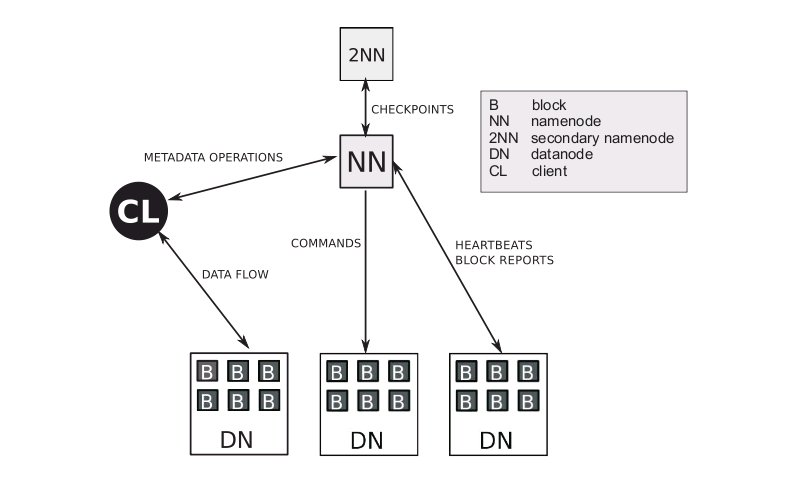
\includegraphics[scale=.6]{figuras/HDFS-arquitetura-2.jpg}
      \caption{Arquitetura do HDFS \cite{TR-IC-10-24}}
      \label{fig6:hfs}
    \end{figure} 

Os DataNodes respondem aos pedidos de leitura e escrita de clientes do
sistema de arquivos e também executam a criação, eliminação e
replicação de blocos sob instrução do NameNode. O número de réplicas é
geralmente 3. A 1$^a$ réplica fica local, no mesmo nó do código do
cliente. A 2$^a$ réplica fica em um nó em outro \emph{rack} e a 3$^a$
réplica fica nesse último \emph{rack} em outro nó. As 2$^a$ e 3$^a$
réplicas não são locais ao bloco replicado.

O NameNode e DataNode são partes do \emph{software} projetado para
rodar em \emph{commodity hardware}. Essas máquinas normalmente
executam um sistema operacional GNU/Linux.

HDFS é construído usando a linguagem Java. Qualquer máquina que suporte
Java pode executar o NameNode ou o DataNode \cite{Hadoop:2010}.

\vspace*{2cm}
\begin{figure}[h]
  \centering
  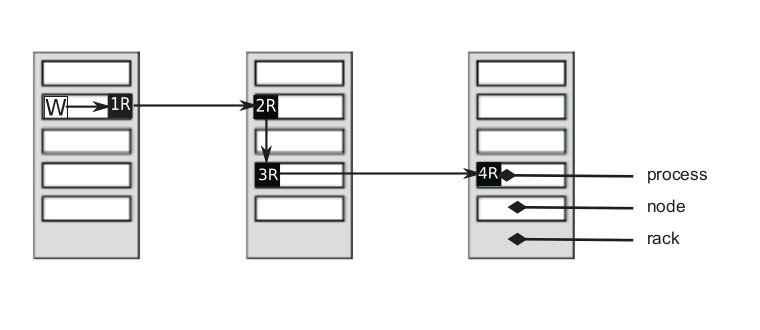
\includegraphics[scale=.5]{figuras/HDFS-arquitetura-replicacao-2.jpg}
  \caption{Arquitetura do HDFS - Datanodes e Blocos \cite{White:2009}}
  \label{fig7:hfs}
\end{figure} 

Os protocolos do HDFS usam o protocolo TCP/IP. O cliente fala o
protocolo ClientProtocol com o NameNode através de uma porta. Os
DataNodes falam o protocolo DataNodeProtocol com o NameNode. Esses
protocolos executam uma \emph{Remote Procedure Call} (RPC). O NameNode
não inicia chamadas RPCs. Ele responde a chamadas RPCs feitas pelo
DataNodes e pelos clientes.

\section{Codificação por Apagamento}

Existe uma nova característica proposta em 2009 para implementação de
uma camada de codificação por apagamento no Hadoop utilizando
XOR (RAID-5)~\cite{HDFS-503:2010} e uma mais recente utilizando códigos
RS~\cite{MR-1969:2010}. A inclusão da codificação por apagamento foi proposta com o
objetivo de reduzir o tamanho do armazenamento do HDFS.

A versão atual do Hadoop não utiliza apenas a técnica de replicação
\cite{White:2009} para obter disponibilidade e confiabilidade de
dados. Ela pode ser configurada para usar também  codicação XOR (RAID-5) e RS.

No HDFS, a codificação RS \emph{default} é (8, 5) e a XOR \emph{default} é (6, 5).  Logo, toleram até $l=3$ e até $l=1$ falhas, respectivamente, por \emph{stripe} de 5 blocos ($k=5$) com sobrecarga de $B=1.6$ e de $B=1.2$, respectivamente. Ambas foram projetadas sob o corpo $GF(2^8)$. O polinômio primitivo dessa codificação RS é $x^8\ +\ x^4\ +\ x^3\ +\ x^2\ +\ 1$.

Na codificação XOR, é possível configurar o número de blocos por \emph{stripe}. Já na codificação RS, tanto o número de blocos por \emph{stripe} e como o número de blocos de paridade são configuráveis.

\subsection{Algoritmos da Camada RAID}

Exemplo do algoritmo de codificação

O tamanho da \emph{stripe} é 5 blocos e existe um arquivo $/a/arquivo.txt$ com exatamente 5 blocos. Nesse caso, o algoritmo de codificação da camada RAID faz o seguinte:

\begin{verbatim}
bloco[0] = primeiro bloco
bloco[1] = segundo bloco
bloco[2] = terceiro bloco
bloco[3] = quarto bloco
bloco[4] = quinto bloco

bloco_paridade = iniciado com 0 em todos os bytes

para i de 0 até número de bytes em um bloco:
   para j de 0 até 4:
      bloco_paridade = bloco_paridade xor bloco[j][i]

para i de 0 até 4:
   escreva bloco_paridade no arquivo /raid/a/arquivo.txt
\end{verbatim}

\subsection{Algoritmos da Camada RS}

Exemplo do algoritmo de codificação

O tamanho da \emph{stripe} é 5 blocos, são 3 blocos de paridade, o polinômio primitivo é $x^8 + x^4 + x^3 + x^2 + 1$ e existe um arquivo $/a/arquivo.txt$ com exatamente 5 blocos. Nesse caso, o algoritmo de codificação da camada RS faz o seguinte:

\begin{verbatim}
// polinômio primitivo g representado por 285
g = x^8 + x^4 + x^2 + x + 1 
m = 8
k = 5
i = 0
L = m-k
j = 0

bloco[0] = primeiro bloco
bloco[1] = segundo bloco
bloco[2] = terceiro bloco
bloco[3] = quarto bloco
bloco[4] = quinto bloco

enquanto j >= L faça
   // para GF = 2
   // x^0 representado por 1; x^1 por 2; x^2 por 4; x^3 por 8; 
   // x^4 por 16; x^5 por 32; x^6 por 64; x^7 por 128;
   a = x^j
   i = 0
   bloco_paridade[j] = iniciado com 0 em todos os bytes
   enquanto i >= k faça
      r = novo bloco
      resto(g, a, bloco[i], r)
      bloco_paridade[j] = bloco_paridade[j] xor r
      i++
   j++
   
para j de 0 até L
   escreva bloco_paridade[j] no arquivo /raidrs/a/arquivo.txt

resto (g, a , bloco, r)
   para i de 0 até número de bytes em um bloco:
      r[i] = resto(g, a, bloco[i])

resto (g, a, b)
retorna resto = (byte) rem (g(b), a(b))
   
\end{verbatim}
